\documentclass[a2paper, 12pt]{article}
\usepackage[font={huge, bf}]{caption}
\usepackage{fontspec}
\setmainfont{Arial}
\usepackage{subcaption}
\usepackage{graphicx}
\usepackage{tikz}
\usepackage{tikzsymbols}
\usetikzlibrary{calc,patterns,shapes.geometric}
\usepackage{float}
\usepackage{pdflscape}
\usepackage{geometry}
\geometry{landscape, margin=2cm}
\captionsetup[subfigure]{justification=justified,singlelinecheck=false}
\pagestyle{empty}

\def\centerarc[#1](#2)(#3:#4:#5){\draw[#1] ($(#2)+({#5*cos(#3)},{#5*sin(#3)})$) arc (#3:#4:#5);}

\begin{document}
	\vspace*{\fill}
	\begin{figure}[!htbp]
		\centering
		\begin{subfigure}[b]{0.48\textwidth}
			\caption{Figure 1}
			\centering
			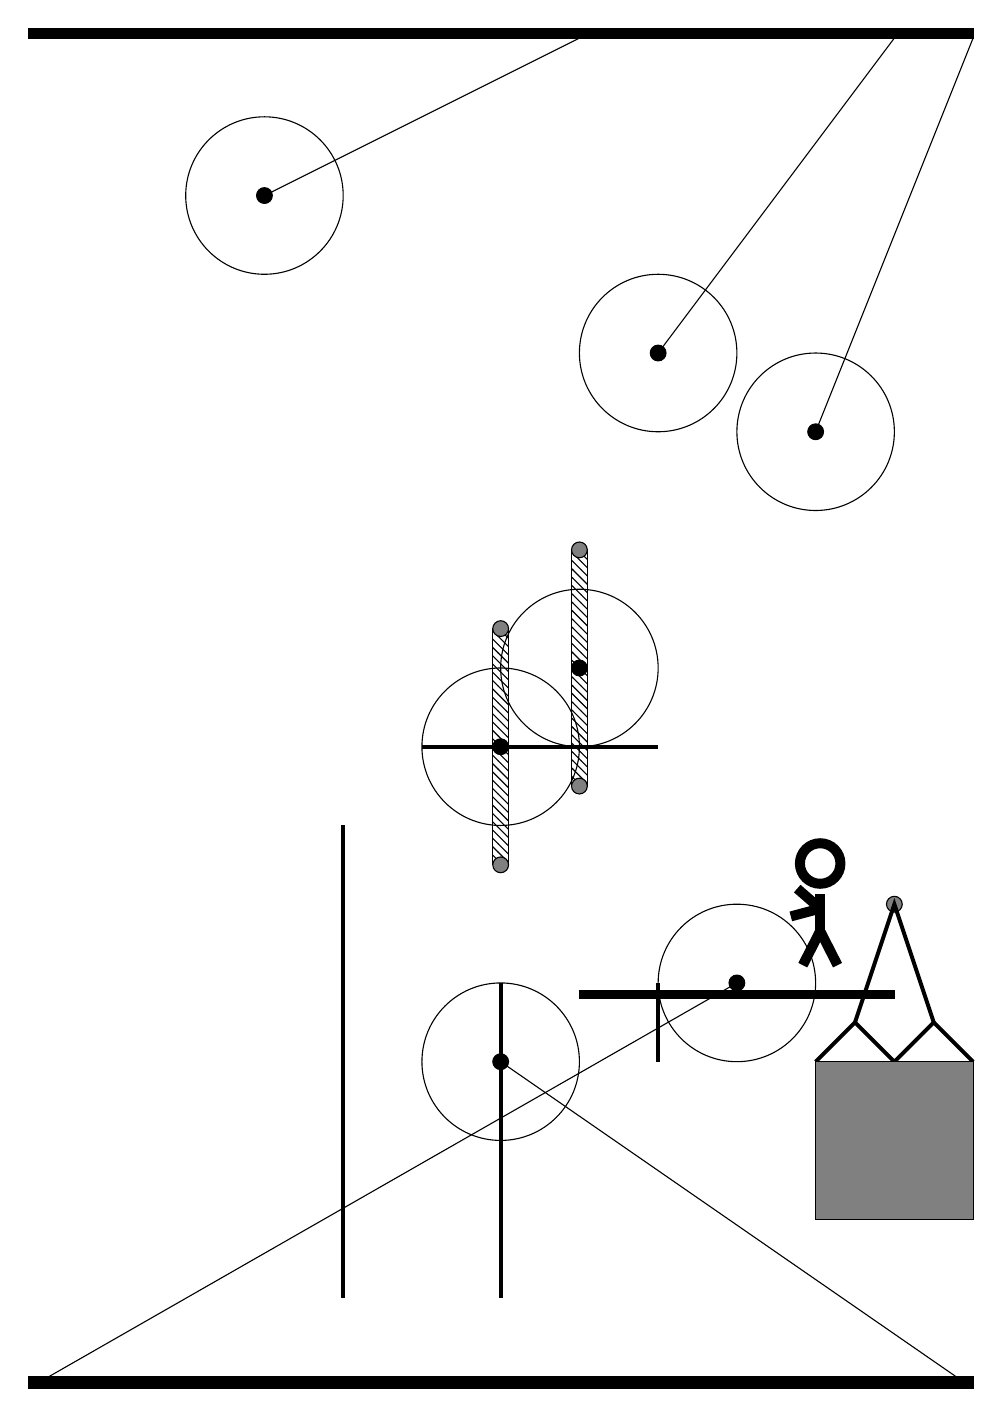
\begin{tikzpicture}
				\draw[fill=black] (-2, 14) rectangle (10, 14.125);
				
				\draw (1,12) circle (1);
				\draw[fill=black] (1,12) circle (0.1);
				\draw (5,14.0) -- (1,12);
				
				\draw (8,9) circle (1);
				\draw[fill=black] (8,9) circle (0.1);
				\draw (10,14.0) -- (8,9);
				
				\draw (7,2) circle (1);
				\draw[fill=black] (7,2) circle (0.1);
				\draw (-2,-3.15) -- (7,2);
				
				\draw (4,5) circle (1);
				\draw[fill=black] (4,5) circle (0.1);
				\draw[pattern=north west lines, pattern color=black] (3.9,6.5) rectangle (4.1,3.5);
				\draw[fill=black!50] (4,6.5) circle (0.1);
				\draw[fill=black!50] (4,3.5) circle (0.1);
				
				\draw (6,10) circle (1);
				\draw[fill=black] (6,10) circle (0.1);
				\draw (9,14.0) -- (6,10);
				
				\draw (5,6) circle (1);
				\draw[fill=black] (5,6) circle (0.1);
				\draw[pattern=north west lines, pattern color=black] (4.9,7.5) rectangle (5.1,4.5);
				\draw[fill=black!50] (5,7.5) circle (0.1);
				\draw[fill=black!50] (5,4.5) circle (0.1);
				
				\draw (4,1) circle (1);
				\draw[fill=black] (4,1) circle (0.1);
				\draw (10,-3.15) -- (4,1);
				
				\draw[fill=black!50] (9,3) circle (0.1);
				\draw[line width=0.5mm](8.5,1.5) -- (9,3) --  (9.5,1.5);
				\draw[line width=0.5mm](8,1) --  (8.5,1.5) -- (9,1) -- (9.5,1.5) -- (10,1);
				\draw[fill=black!50] (8, 1) rectangle (10, -1);
				
				\draw[line width = 0.5mm] (3,5) -- (6,5);
				\centerarc[line width = 0.5mm](3,4)(90:180:1);
				\draw[line width = 0.5mm] (2,4) -- (2,-2);
				\centerarc[line width = 0.5mm](3,-2)(180:360:1);
				\draw[line width = 0.5mm] (4,-2) -- (4,2);
				\centerarc[line width = 0.5mm](5,2)(0:180:1);
				\draw[line width = 0.5mm] (6,2) -- (6,1);
				\centerarc[line width = 0.5mm](7,1)(180:270:1);
				
				\node at (8, 3) {\scriptsize \Strichmaxerl[10][-41][-165]};
				\draw[fill=black] (5, 1.9) rectangle (9, 1.8);
				
				\draw[fill=black] (-2, -3) rectangle (10, -3.15);
			\end{tikzpicture}
		\end{subfigure}
		\hfill
		\begin{subfigure}[b]{0.48\textwidth}
			\caption{Figure 2}
			\centering
			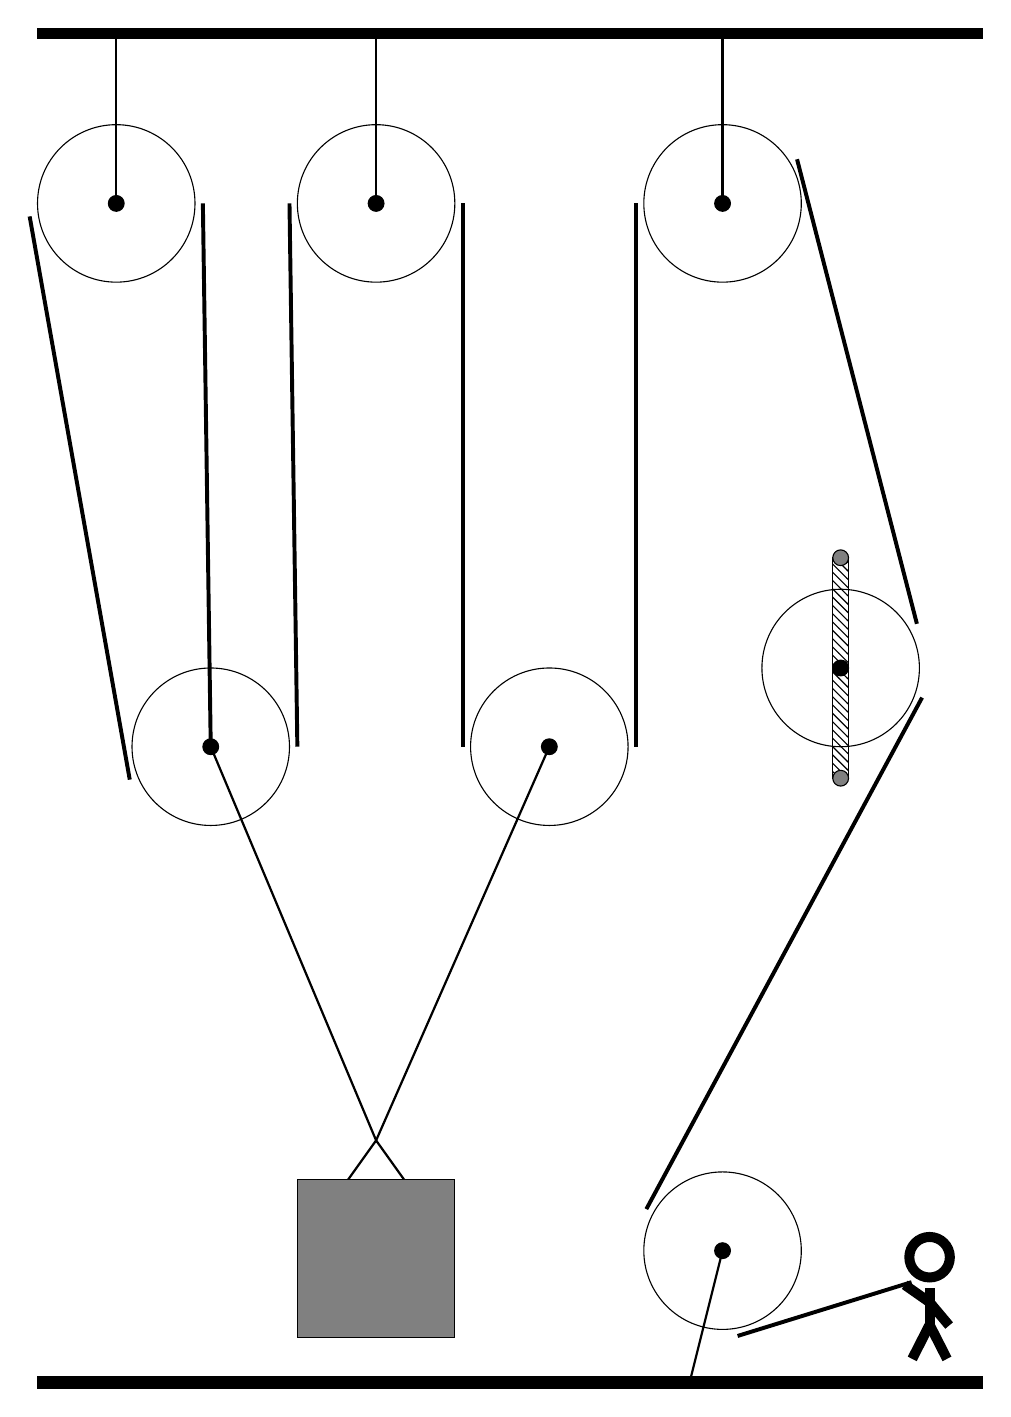
\begin{tikzpicture}
				\draw[fill=black] (-2, 14) rectangle (10, 14.125);
				
				\draw (-1, 11.9) circle (1);
				\draw[fill=black] (-1, 11.9) circle (0.1);
				\draw[thick] (-1, 11.9) -- (-1, 14);
				
				\draw (2.3, 11.9) circle (1);
				\draw[fill=black] (2.3, 11.9) circle (0.1);
				\draw[thick] (2.3, 11.9) -- (2.3, 14);
				
				\draw (6.7, 11.9) circle (1);
				\draw[fill=black] (6.7, 11.9) circle (0.1);
				\draw[thick] (6.7, 11.9) -- (6.7, 14);
				
				\draw (0.2, 5) circle (1);
				\draw[fill=black] (0.2, 5) circle (0.1);
				
				\draw (4.5, 5) circle (1);
				\draw[fill=black] (4.5, 5) circle (0.1);
				
				\draw (8.2, 6) circle (1);
				\draw[fill=black] (8.2, 6) circle (0.1);
				\draw[pattern=north west lines, pattern color=black] (8.1, 7.4) rectangle (8.3, 4.6);
				\draw[fill=black!50] (8.2, 7.4) circle (0.1);
				\draw[fill=black!50] (8.2, 4.6) circle (0.1);
				
				\draw (6.7, -1.4) circle (1);
				\draw[fill=black] (6.7, -1.4) circle (0.1);
				\draw[thick] (6.7, -1.4) -- (6.3, -3);
				
				\draw[thick] (0.2, 5) -- (2.3, 0)  -- (4.5, 5);
				\draw[thick]  (1.8, -0.7) -- (2.3, 0) -- (2.8, -0.7);
				\draw[fill=black!50] (1.3, -0.5) rectangle (3.3, -2.5);
				\draw[line width=0.5mm] (0.2, 5) -- (0.1, 11.9);
				\centerarc[line width=0.5mm](-1, 11.9)(0:200:1.1);
				\draw[line width=0.5mm] (-2.1, 11.735) -- (-0.8285, 4.582);
				\centerarc[line width=0.5mm](0.2, 5)(200:360:1.1);
				\draw[line width=0.5mm](1.3, 5) -- (1.2, 11.9);
				\centerarc[line width=0.5mm](2.3, 11.9)(0:180:1.1);
				\draw[line width=0.5mm] (3.4, 11.9) -- (3.4, 5);
				\centerarc[line width=0.5mm](4.5, 5)(180:360:1.1);
				\draw[line width=0.5mm] (5.6, 5) -- (5.6, 11.9);
				\centerarc[line width=0.5mm](6.7, 11.9)(30:180:1.1);
				\draw[line width=0.5mm](7.646, 12.461) -- (9.168, 6.561);
				\centerarc[line width=0.5mm](8.2, 6)(160:211:-1.1);
				\draw[line width=0.5mm](9.2337, 5.6238) -- (5.732, -0.872);
				\centerarc[line width=0.5mm](6.7, -1.4)(150:280:1.1);
				\draw[line width=0.5mm](6.891, -2.4833) -- (9.1, -1.8);
				
				\node at (9.3, -2) {\scriptsize \Strichmaxerl[10][-35][-50]};
				
				\draw[fill=black] (-2, -3) rectangle (10, -3.15);
			\end{tikzpicture}
		\end{subfigure}
	\end{figure}
		\vspace*{\fill}
\end{document}